\begin{frame}
  \frametitle{Storage Layer Representation}
  \begin{itemize}
    \uncover<1->{  \item In the storage layer,
      \begin{itemize}
      \item edge directionality does \textbf{not} exist
      \item connected vertices store information about each other
      }
    \end{itemize}
    \uncover<2->{
    \item Bi-directional edge traversal speeds up query performance
    \end{itemize}
  }
  \uncover<3->{
    \begin{figure}
      \centering
      \begin{tikzpicture}[node distance=2cm,scale=0.6,every node/.style={transform shape}]

  \record(
  0,
  \small{\texttt{a:Person}},
  \small{\texttt{name:Tolkien}},
  $\boldsymbol{\rightarrow}$ \textbf{\small{\texttt{wrote b}}},
  \texttt{edge},
  \texttt{edge}
  );

  \record(
  -1,
  \small{\texttt{b:Book}},
  \texttt{property},
  \small{\texttt{title:The \hspace{-0.15cm} Hobbit}},
  $\boldsymbol{\leftarrow}$ \textbf{\small{\texttt{written by a}}},
  \texttt{edge}
  );

  \record(-2,
  \small{\texttt{vertex id}},
  \texttt{property},
  \texttt{property},
  \texttt{edge},
  \texttt{edge}
  );


  \spaceRecord(-3)

  \record(-4,
  \small{\texttt{vertex id}},
  \texttt{property},
  \texttt{edge},
  \texttt{edge},
  \texttt{edge}
  );

\end{tikzpicture}

      \caption{Edge storage layer representation}
    \end{figure}
  }
\end{frame}